\clearpage
\subsection{Исследование свойств спроектированной нелинейной СПС}
На первом этапе нами была синтезирована СПС без учета нелинейности с линией скольжения  $S_1$, проходящей через начало координат. Затем для синтеза СПС с нелинейным элементом (НЭ) мы синтезировали релейную систему для больших отклонений с линией переключения $S_2=10x_1+6x_2+d$, где значение d определяет координаты точки пересечения линий $S_1$ и $S_2$. Значение $d$ определяет характер процесса в СПС на завершающей стадии движения. Для получения требуемого вида процесса и улучшения показателей системы коэффициенты усиления были скорректированы. Структурная схема для моделирования представлена на  рис.\ref{fig:sim_final_VSS}. 
\begin{figure}[!h]\centering
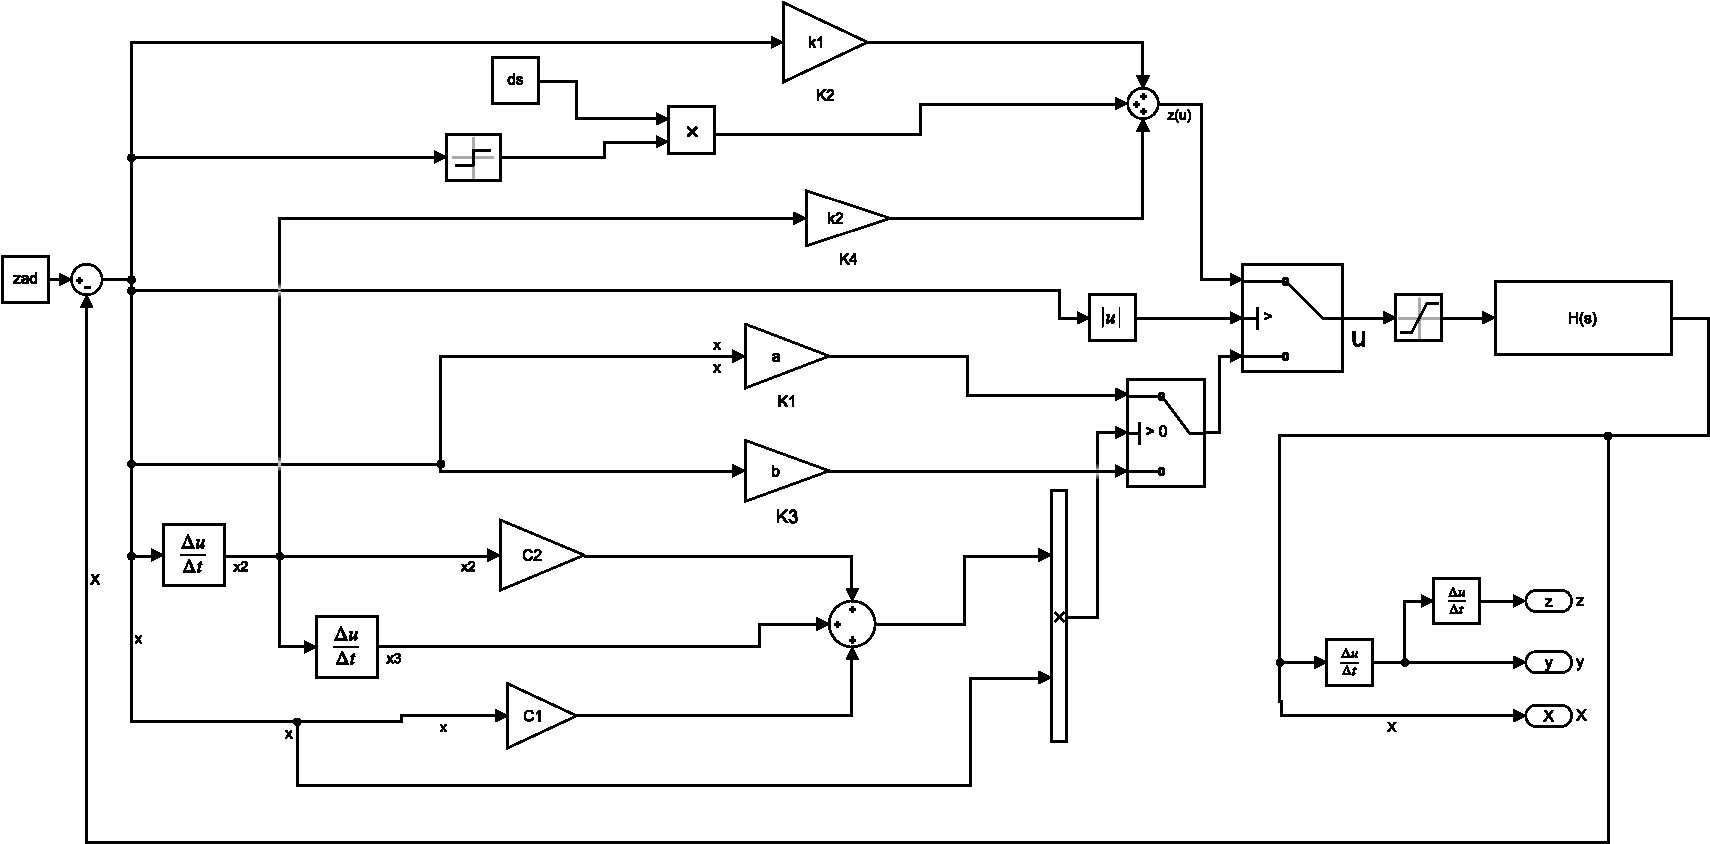
\includegraphics[width=1.0\linewidth]{images/sim_final_VSS}
\caption{Структурная схема нелинейной СПС.}\label{fig:sim_final_VSS}
\end{figure}

Рассмотрим влияние параметров схемы на ПП системы.
Начнем с коэффициентов $K_1,K_2$, они работают при отклонении системы "в большом".
Переходные процессы для разных значений этих параметров на рис.\ref{fig:final_VSS_PWM_k2},графики на всем интервале времени практически не изменяются, только в конце ПП при переключении систем управления появляются различия. Для более детального рассмотрения поакзана приближенная картинка на рис. \ref{fig:final_VSS_PWM_k2_zoom}.
Они представлят собой коэффициенты пропорционального и дифференциального регулятора соответственно.
Соответственно влияют они на систему также, как и коэффициенты ПД-регулятора в пункте \ref{title:PDR}: $k_1$ --- коэффициент пропорционального звена, влияет на скорость нарастания выходной величины, а $k_2$ --- коэффициент дифференцирующего звена, влияет на колебательность системы.
При этом при разных сочетаниях коэффициентов время ПП практически не улучшается и наилучшее время составляет $133.46$ сек.
\begin{figure}[!h]\centering
	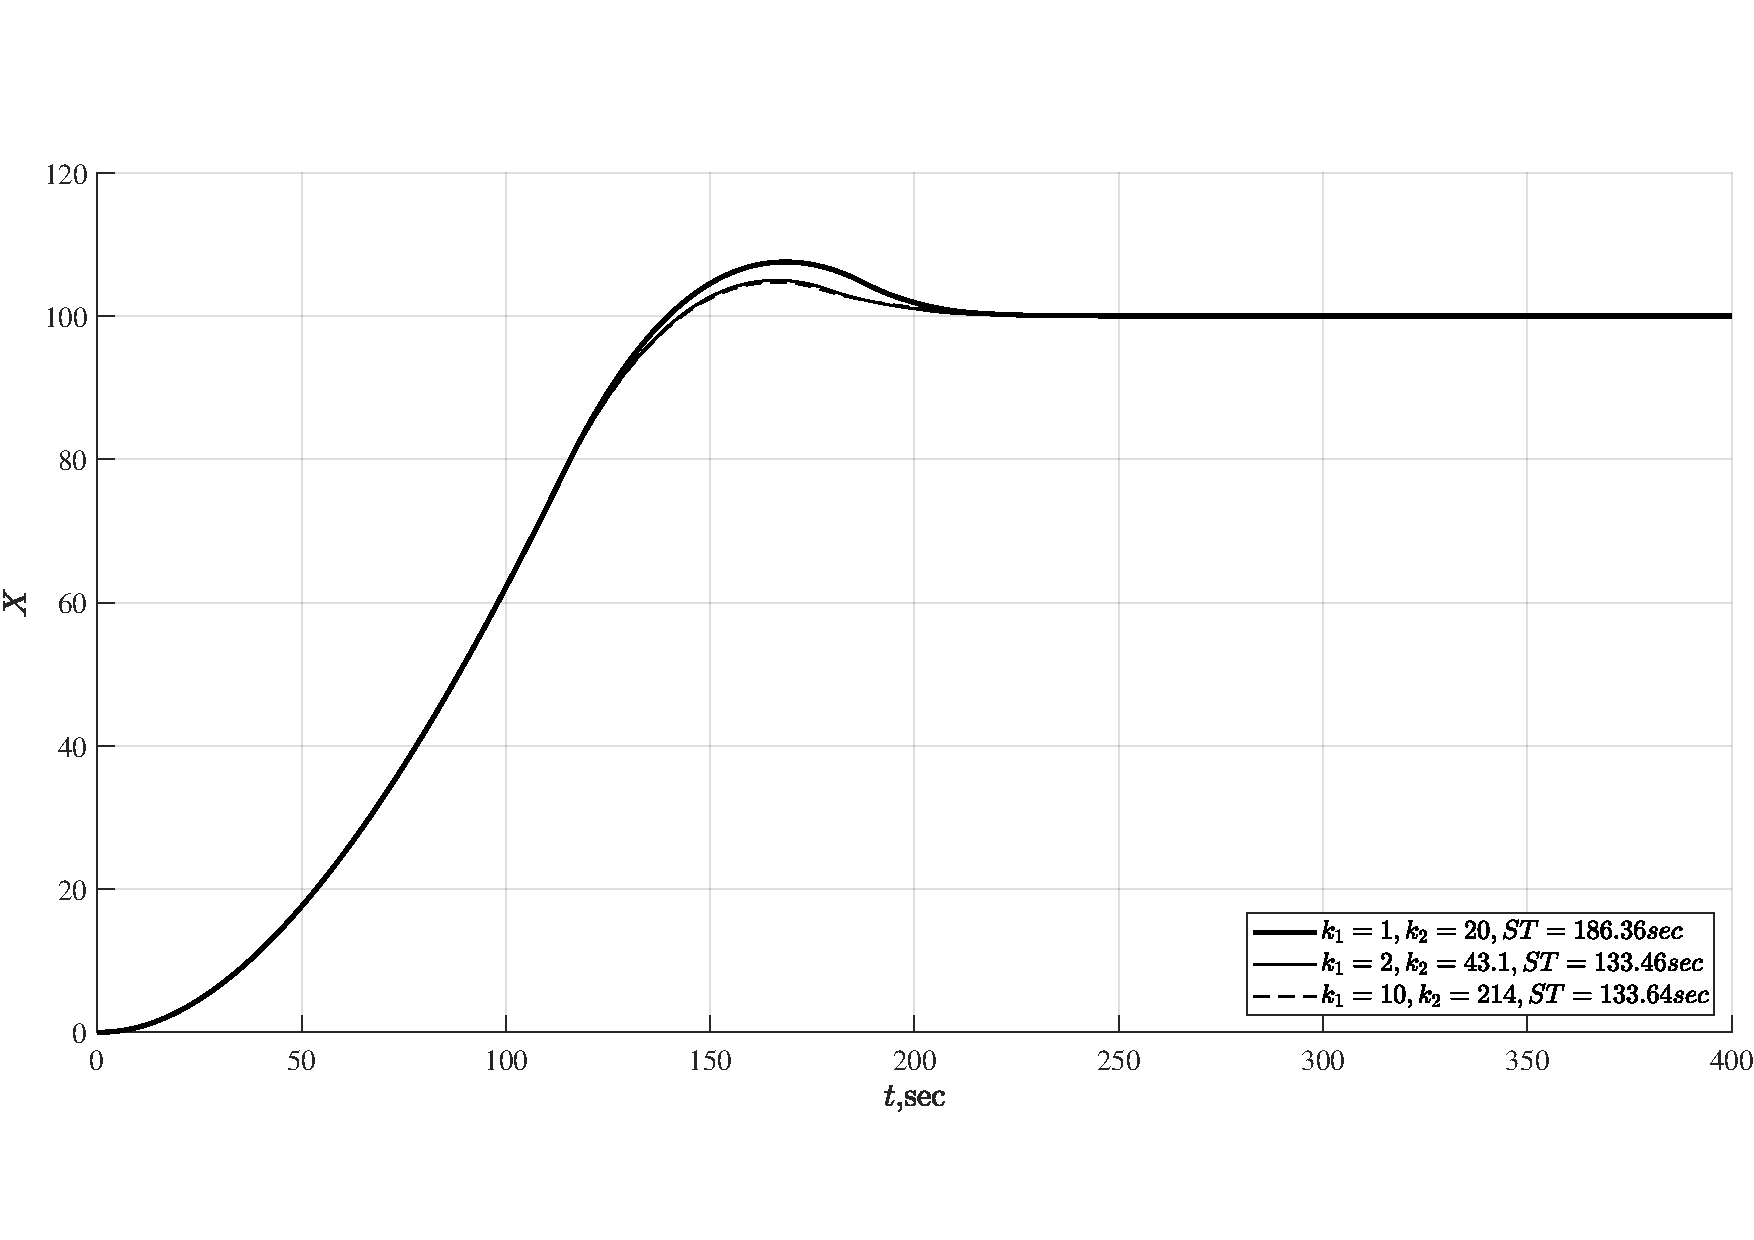
\includegraphics[width=1\linewidth]{images/final_VSS_PWM_k2}
	\caption{ Графики ПП при вариации параметров $k_1,k_2$ в <<большом>>.}\label{fig:final_VSS_PWM_k2}
\end{figure}
\begin{figure}[!h]\centering
	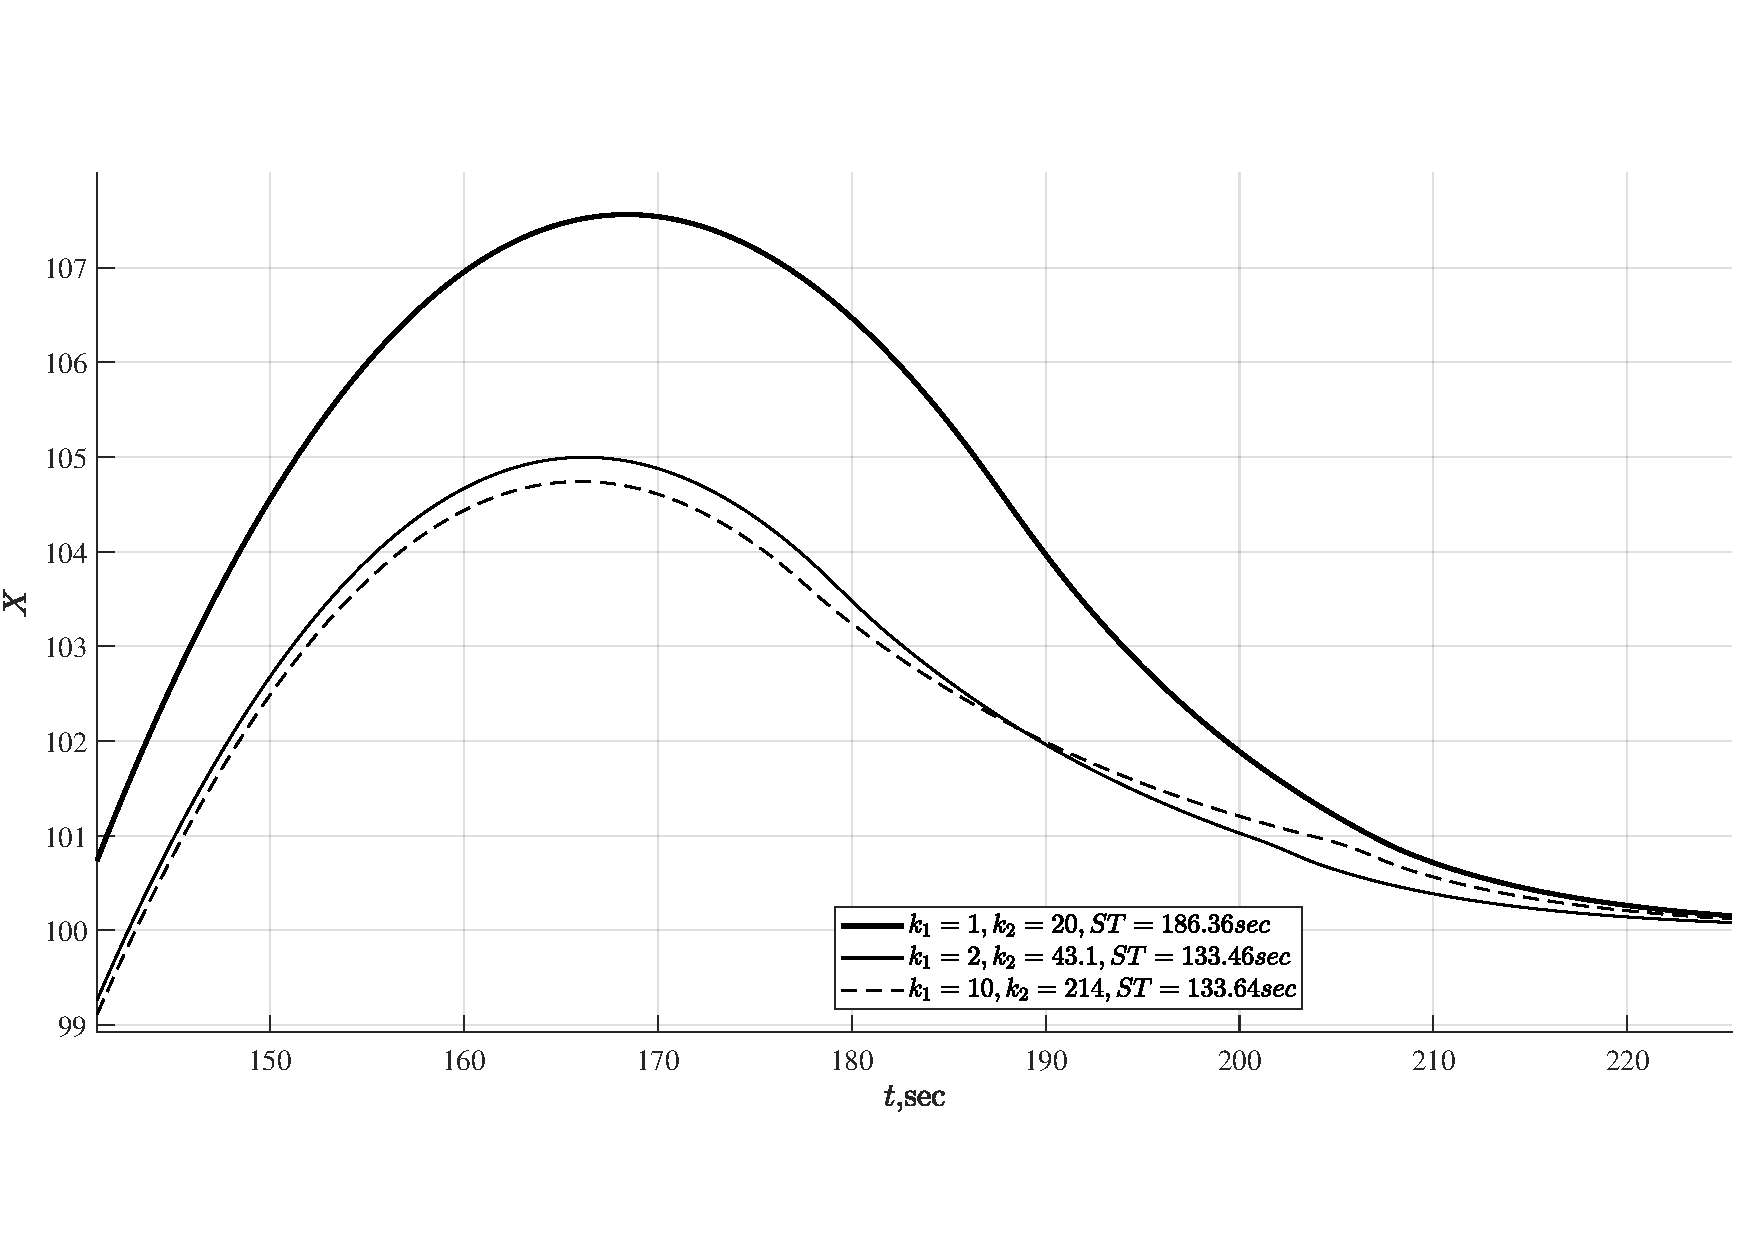
\includegraphics[width=1\linewidth]{images/final_VSS_PWM_k2_zoom}
	\caption{ Приближенный график ПП при вариации параметров $k_1,k_2$.}\label{fig:final_VSS_PWM_k2_zoom}
\end{figure}

Теперь рассмотрим коэффициенты, влияющие на ПП "в малом": $C1,C2,a,b$. Также стоит отметить порог, отвечающий за переключение систем управления (переключение структур) при превышении абсолютными значениями ошибки данного порога. Данный порог определяет в какой момент переключить сруткуру, дргуими словами, он определяет при какие отклонения можно считать "большими", а какие "малыми". Так как при настройке системы отклонение "в малом" устанавливалось равным $1$, то и знаечние порога равно $1$. 
Параметры $a$ и $b$ незначительно влияют на ПП ситемы  при их отклонениях при правильной настройке.
Это можно увидеть на рисунке \ref{fig:final_VSS_PWM_ab}. 
\begin{figure}[!h]\centering
	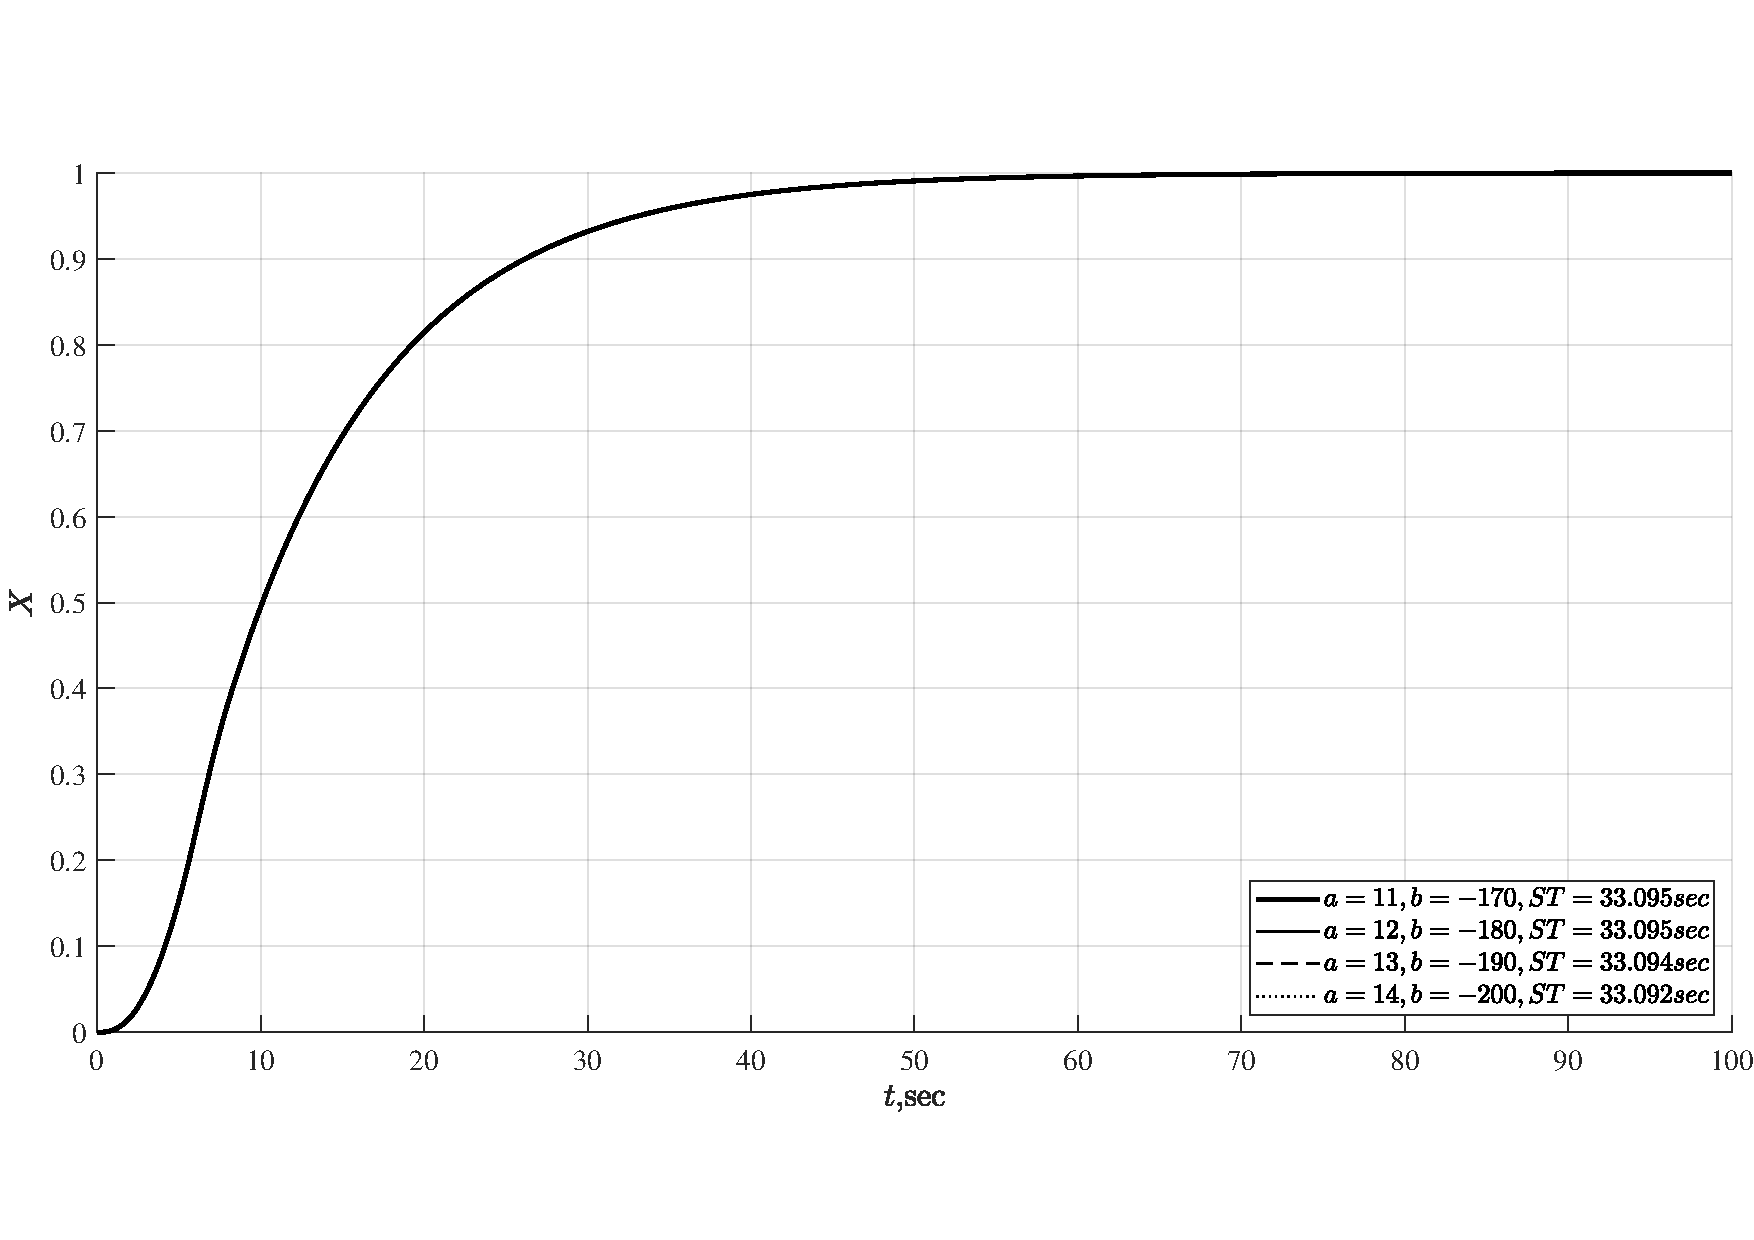
\includegraphics[width=1\linewidth]{images/final_VSS_PWM_ab}
	\caption{ Графики ПП при вариации параметров $a,b$ в <<малом>>.}\label{fig:final_VSS_PWM_ab}
\end{figure}
Параметры $C1$ и $C2$ на колебательность и скорость нарастания. При увеличении $C1$ колебательность и скорость нарастания возрастает, а при увеличении $C2$ колебательность уменьшается. На рис. \ref{fig:final_VSS_PWM_c1c2} ПП ,  соответствующий техническим требованиям, при разных комбинациях параметров (На рис.\ref{fig:final_VSS_PWM_c1c2_zoom} в увеличенном масштабе). 
\begin{figure}[!h]\centering
	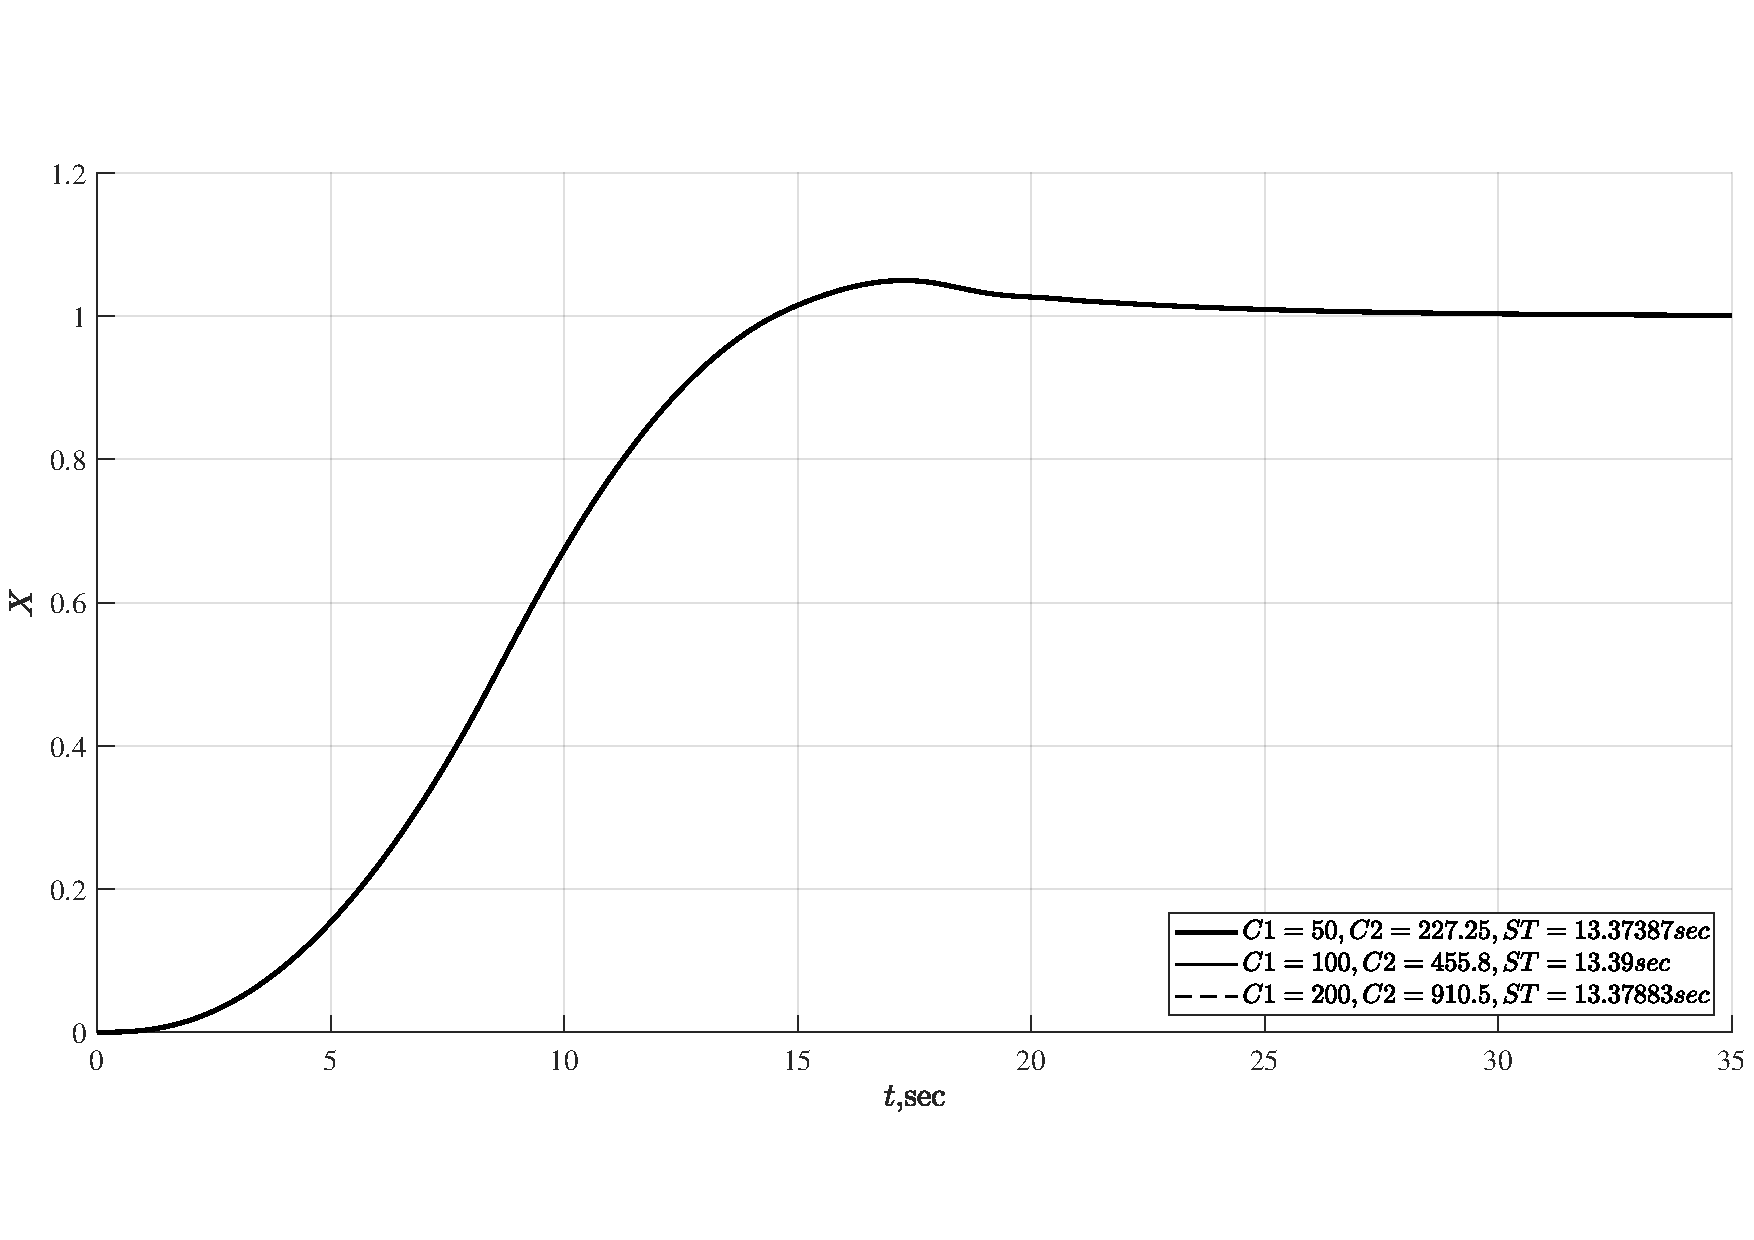
\includegraphics[width=1\linewidth]{images/final_VSS_PWM_c1c2}
	\caption{ Графики ПП при вариации параметров $C1,C2$ в <<малом>>.}\label{fig:final_VSS_PWM_c1c2}
\end{figure}
\begin{figure}[!h]\centering
	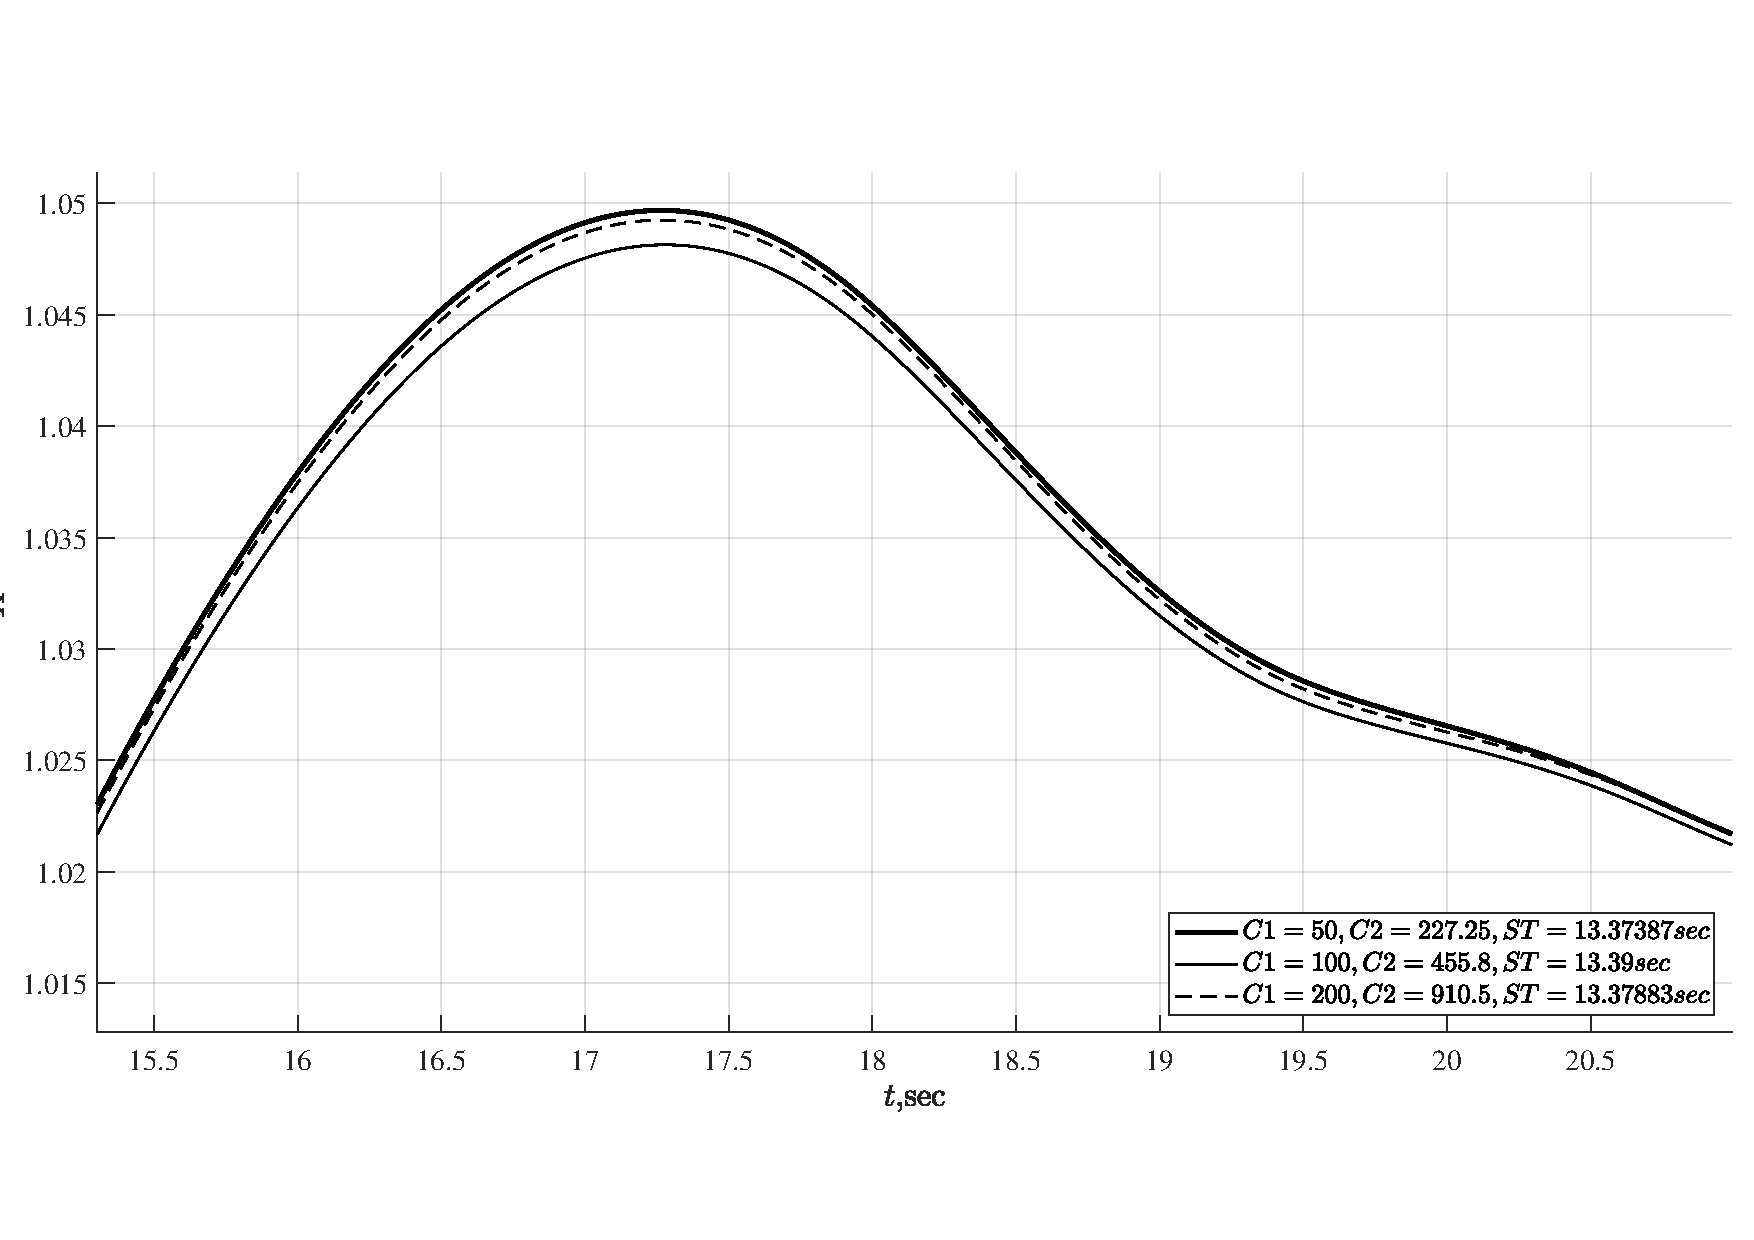
\includegraphics[width=1\linewidth]{images/final_VSS_PWM_c1c2_zoom}
	\caption{ Графики ПП при вариации параметров $C1,C2$ в <<малом>>.}\label{fig:final_VSS_PWM_c1c2_zoom}
\end{figure}

Исследуем движение фазовых координат во времени посредством моделирования процессов в системе при отклонении системы от состояния равновесия. Фазовые траектории в системе на рис.\ref{fig:final_VSS_ft_VSS_final_2_mal}. 
В дополнение на рис.\ref{fig:final_VSS_sv_VSS_final_mal} указано изменение выходной переменной и её производной.
В табл.\ref{tab:tab_settlinhtime_VSS_final} отобразим время регулирования при разных значениях параметров

\begin{table}[!h] \centering
    \caption{Сравнение результатов} \label{tab:tab_settlinhtime_VSS_final}
    \begin{tabular}{|c|c|c|c|c|c|c|c|c|c|c|}
        \hline
        zad & отклонение & $\alpha$ & $\beta$ & $C_1$ & $C_2$ & $k_1$ & $k_2$ & $ds$ & $sw1$ & $t_p$ \\ \hline
        $1$ &в малом& $14$ & $-200$ & $50$ & $227$ & $2$ & $43.1$ & $1$ & $1$ & $13.5$ \\ \hline
        $100$ &в большом& $14$ & $-200$ & $50$ & $227$ & $2$ & $43.1$ & $1$ & $1$ & $167$ \\ \hline
    \end{tabular}
\end{table}
\begin{figure}[!h]\centering
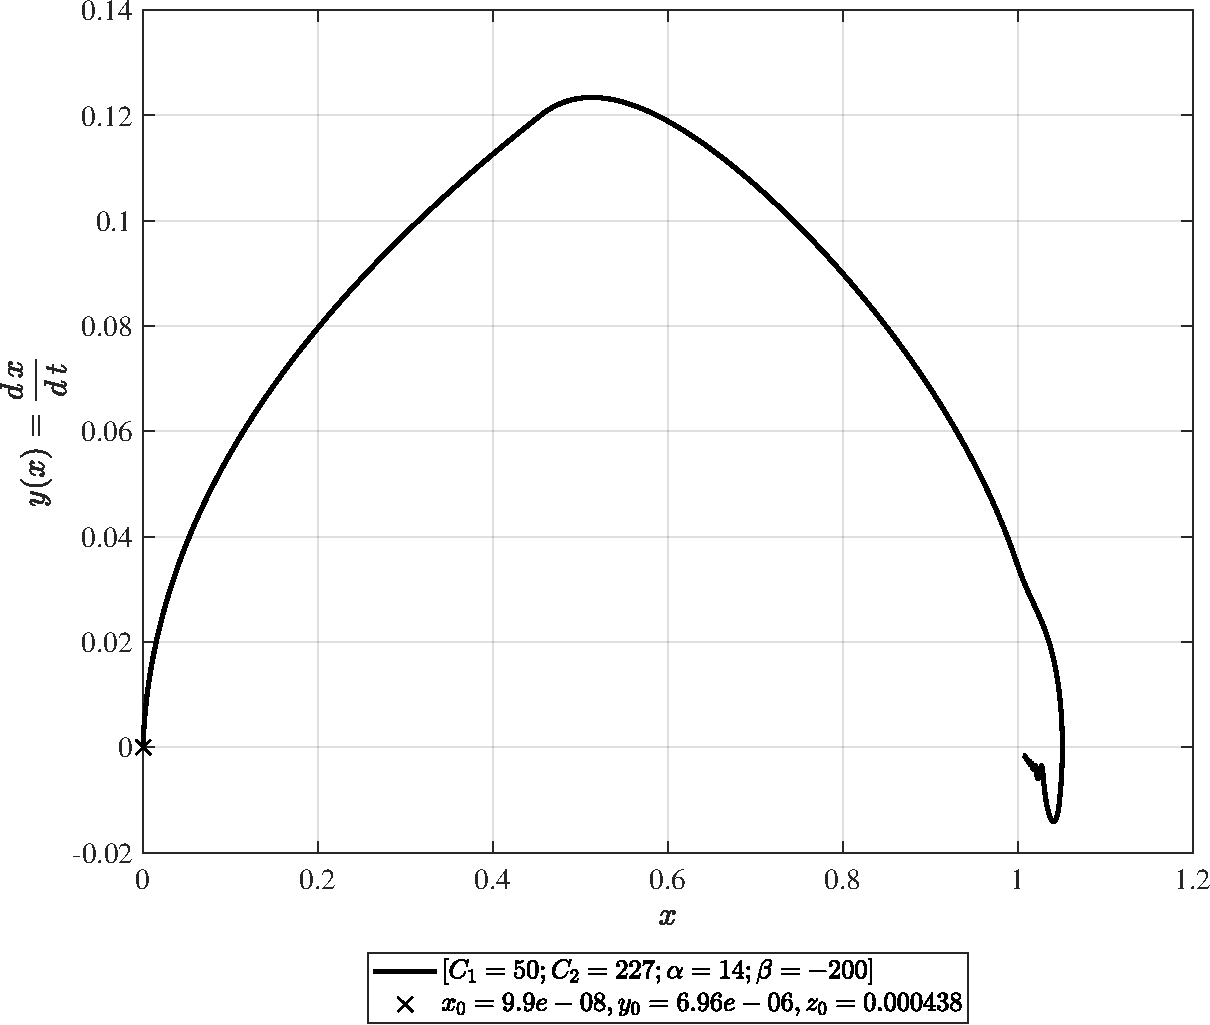
\includegraphics[width=0.7\linewidth]{images/final_VSS_ft_VSS_final_2_mal}
\caption{ Фазовые траектории для системы в <<малом>> с переменной структурой для переменных состояния $x_1,x_2$.}\label{fig:final_VSS_ft_VSS_final_2_mal}
\end{figure}
\begin{figure}[!h]\centering
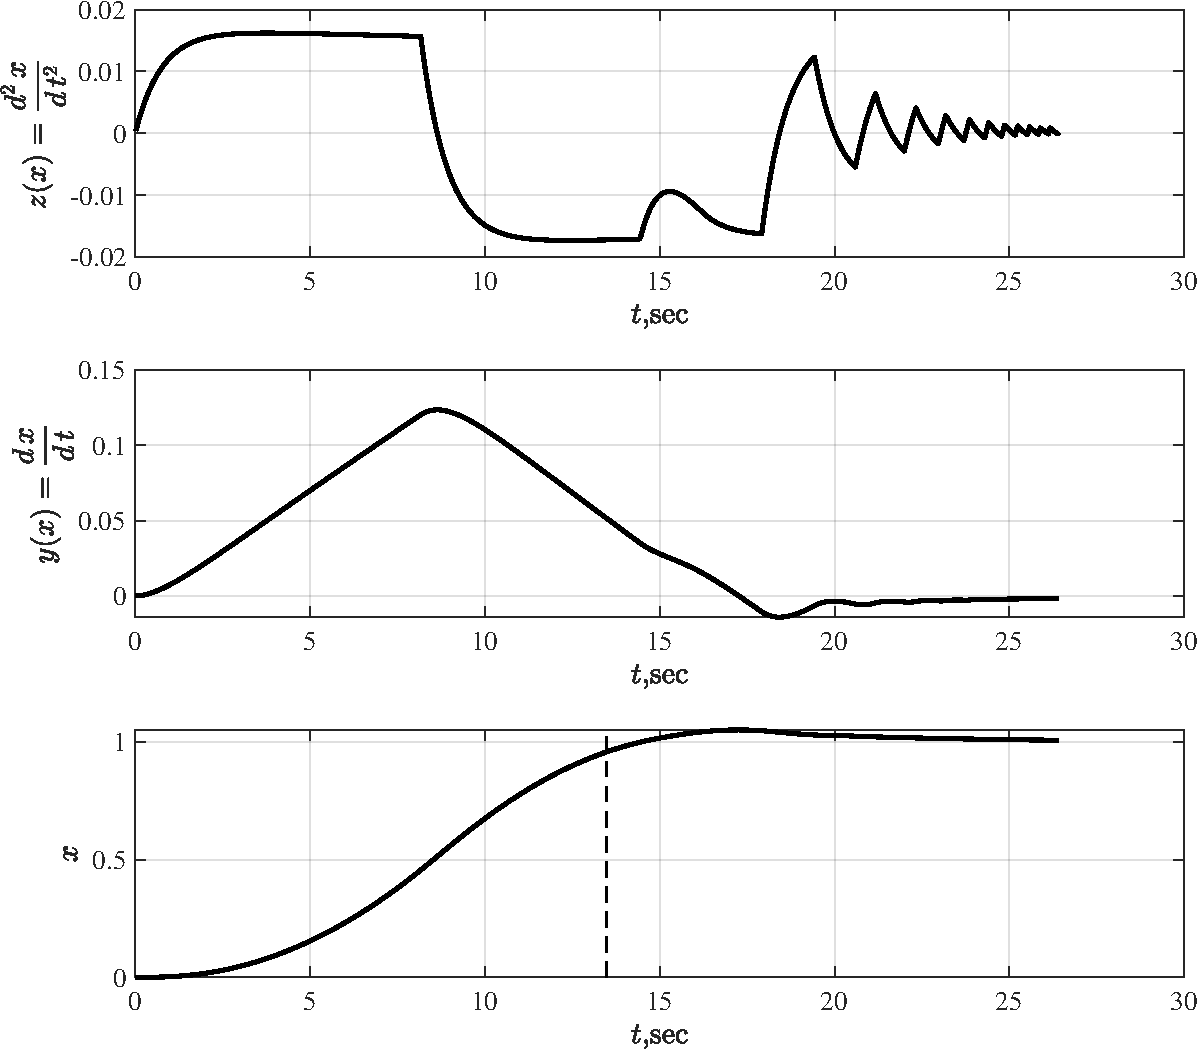
\includegraphics[width=1.0\linewidth]{images/final_VSS_sv_VSS_final_mal}
\caption{ Графики изменения переменных состояния в <<малом>>.}\label{fig:final_VSS_sv_VSS_final_mal}
\end{figure}
\begin{figure}[!h]\centering
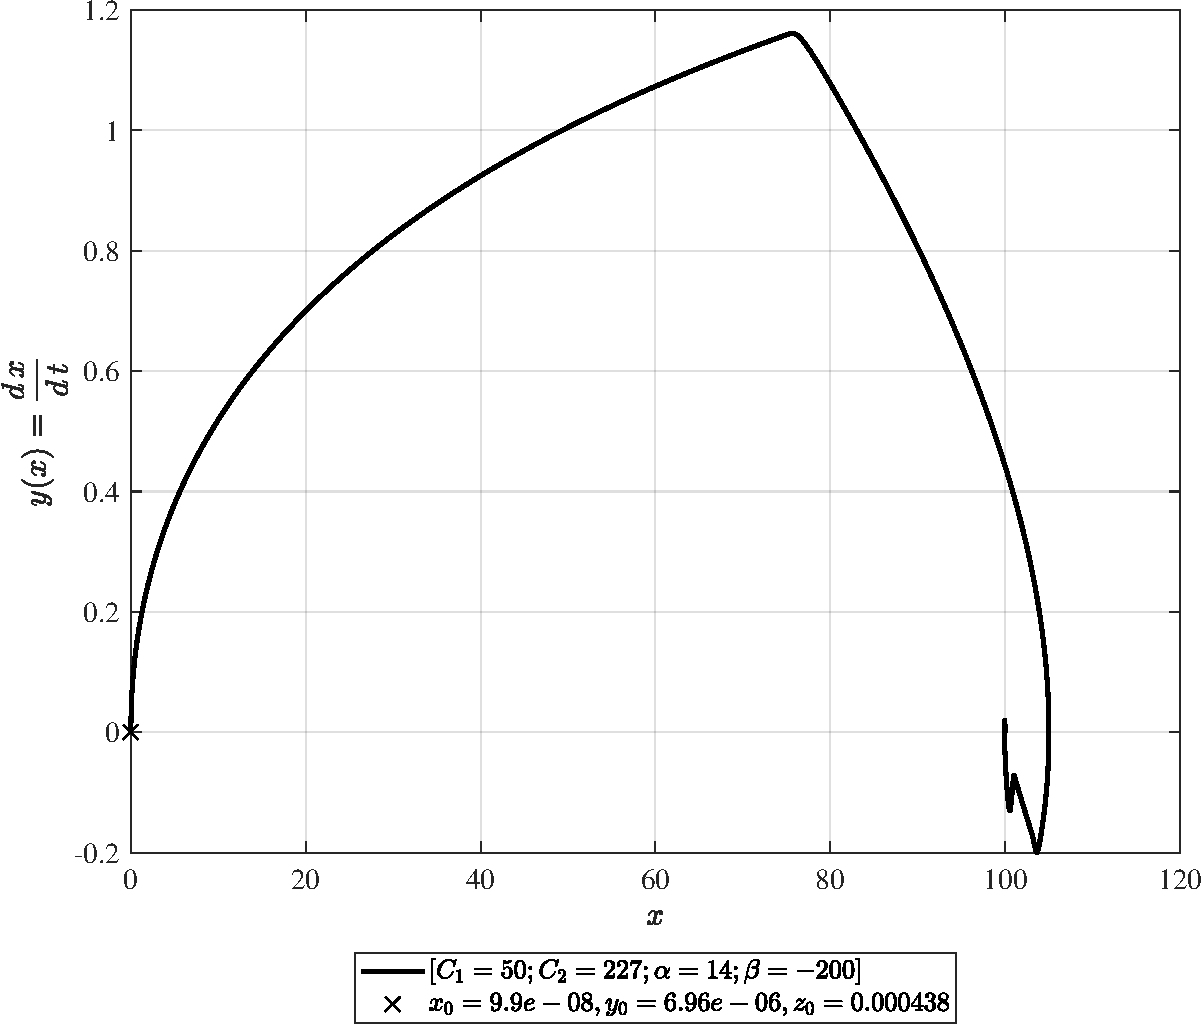
\includegraphics[width=0.7\linewidth]{images/final_VSS_ft_VSS_final_2_bol}
\caption{ Фазовые траектории для системы в <<большом>> с переменной структурой для переменных состояния $x_1,x_2$.}\label{fig:final_VSS_ft_VSS_final_2_bol}
\end{figure}
\begin{figure}[!h]\centering
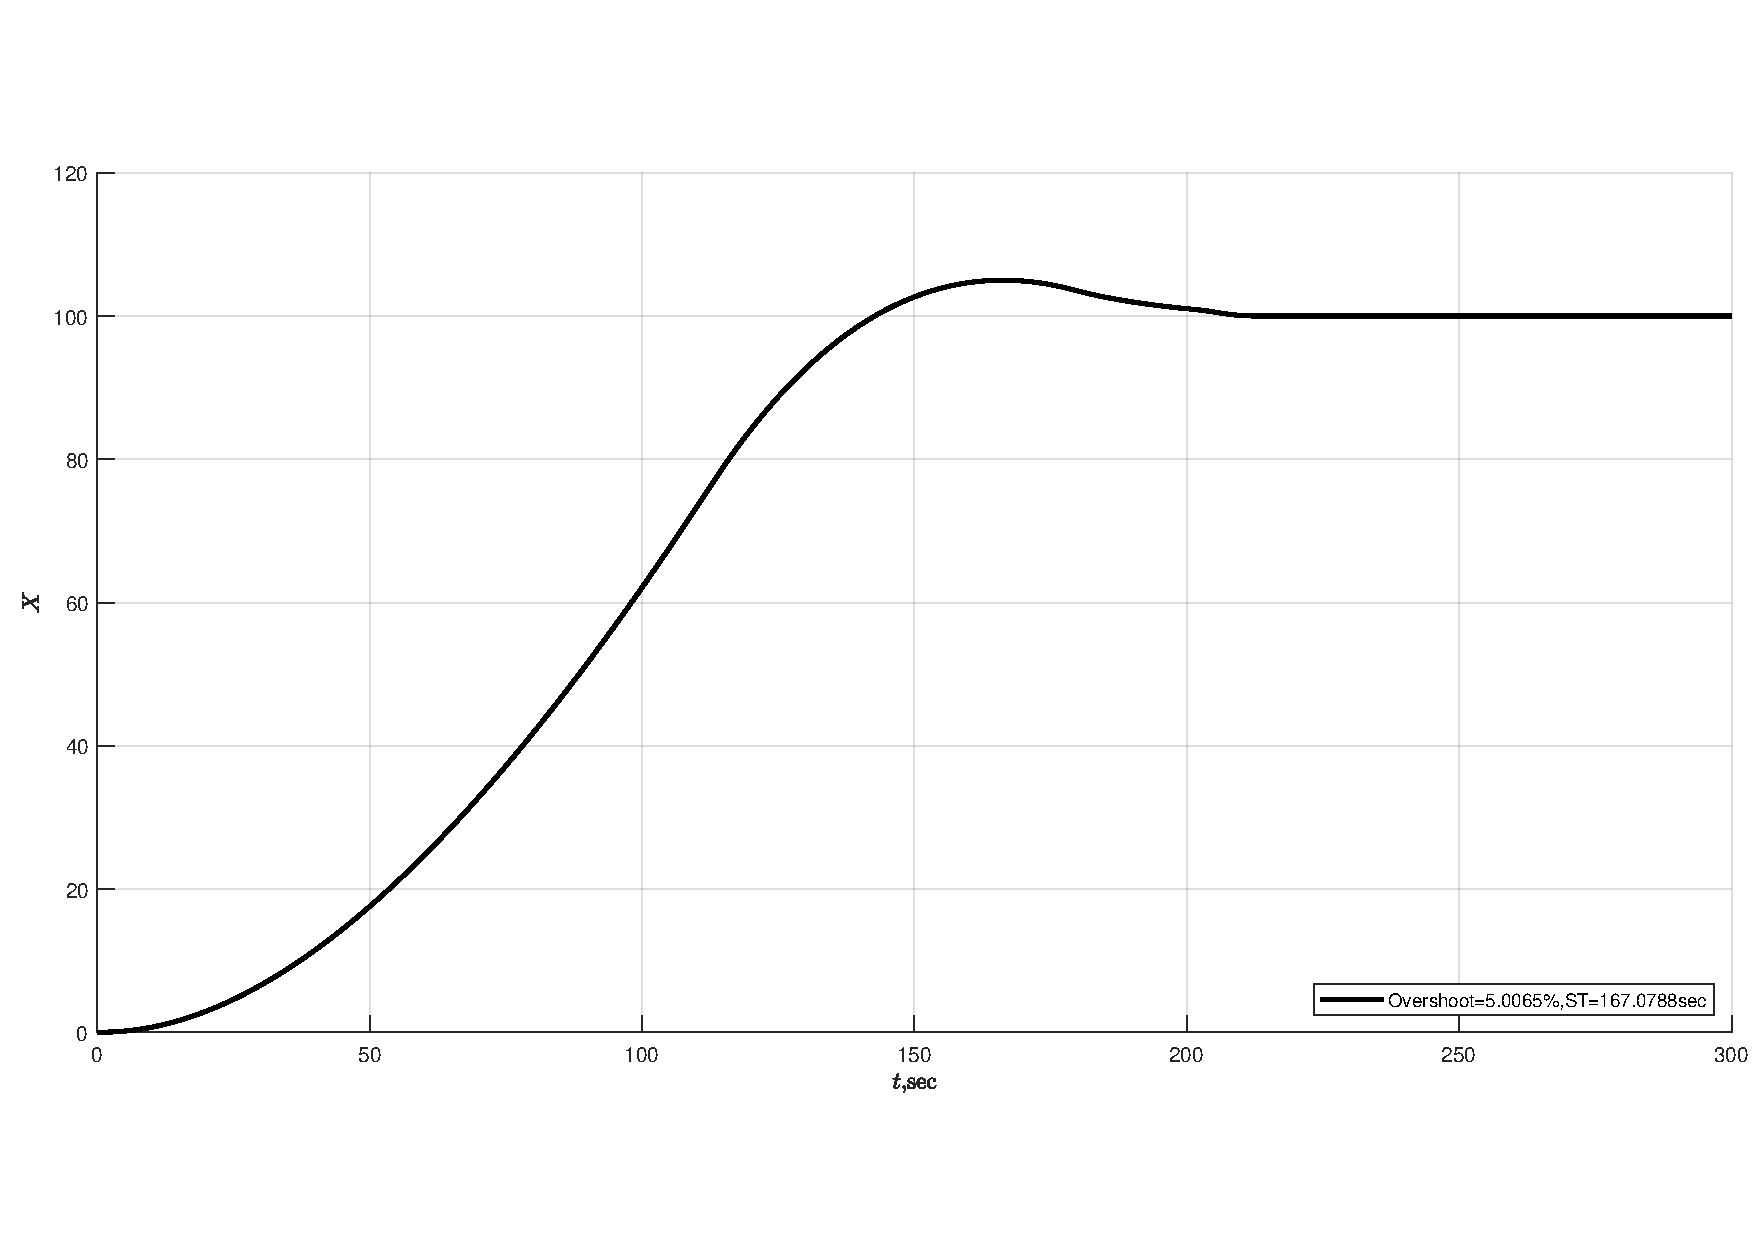
\includegraphics[width=1.0\linewidth]{images/final_VSS_sv_VSS_final_bol}
\caption{ Графики изменения переменных состояния в <<большом>>.}\label{fig:final_VSS_sv_VSS_final_bol}
\end{figure}

Точность поддержания выходной координаты в установившимся режиме составила $\epsilon=0$ – что удовлетворяет заданным требованиям точности $\epsilon\le1$.
